\begin{figure}
\centering
\begin{subfigure}{8cm}
  \centering
  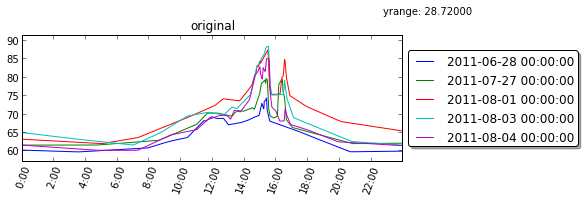
\includegraphics[width=8cm]{fig-original}
  \caption{Original sensor values}
  \label{fig:results-original}
\end{subfigure}%
\begin{subfigure}{8cm}
  \centering
  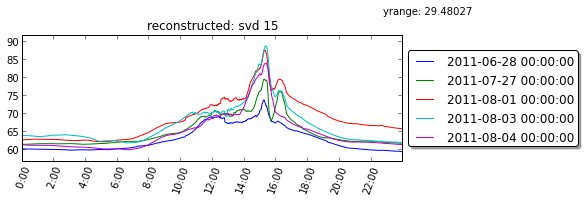
\includegraphics[width=8cm]{fig-reconstructed_svd}
  \caption{Reconstructed sensor values from SVD model}
  \label{fig:results-reconstructed-svd}
\end{subfigure}
\caption{Measurements from a single sensor for 5 days}
\label{fig:results}
\end{figure}
